\chapter{Proposed Protocols}

\label{chap:propprotocol} 

\section{System Model}
Content goes here... 

\subsection{Just Another Subsection} 
Let's discuss about $equation$.


\subsubsection{Just Another subsub: Equation example}
Example 1: BMI Formula \cite{nameofref1}. Syntax $\backslash ref\{eq:1\}$ (Example: \ref{eq:1}) is used to call the equation. Contoh 1: Rumus BMI \cite{nameofref1}. Silahkan gunakan syntax $\backslash ref\{eq:1\}$ (Contoh: \ref{eq:1}) untuk memanggil equation tersebut.

% BMI equation here
\begin{equation}‎
\label{eq:1}
BMI‎ ‎=‎ \frac {we} {he^2}
\end{equation}‎

In equation \ref{eq:2}, it gives another example of how to make use of this $equation$ syntax. Di equation \ref{eq:2} ditunjukkan bagaimana cara lain dalam penggunaan syntax ini.

\begin{equation}‎
\label{eq:2}
K(U, W, C) = 
\mathlarger{\mathlarger{‎‎\sum}}_{i=1}^{N‎}
\mathlarger{\mathlarger{‎‎\sum}}_{k=1}^{K}
\gamma_{ik} (\omega_\alpha \times \omega_\beta)_{x_i} D(x_i,c_k)
\end{equation}‎

For further usage, this $reference$ \footnote{\label{note:latex_wiki_math}\url{https://en.wikibooks.org/wiki/LaTeX/Mathematics}} or $this~one$ \footnote{\label{note:latex_wiki_advmath}\url{https://en.wikibooks.org/wiki/LaTeX/Advanced_Mathematics}} might help you. Untuk informasi lebih detail tentang $equation$, silahkan merujuk ke $sini$ \footnotemark[\ref{note:latex_wiki_math}] atau ke $sana$ \footnotemark[\ref{note:latex_wiki_advmath}].

\subsubsection{Just Another subsub: Algorithm example}
Let's go through how do we write an algorithm and how to $summon$ it into our masterpiece! Berikut merupakan cara penulisan algoritma dan pemanggilannya.


\begin{algorithm}[H]
  \caption{Name of the algorithm, contoh: Algojlo untuk pengguna $U$}
  \label{alg:1}
  \begin{algorithmic}[1]
    
		\Require
      \Statex Data Matrik (A, B) $a \times b \to \phi \times y$.
      \Statex Titik datanya $pn = \{p_1, xp_2, ..., p_l\}$; 
      			$~p_i \to namafunc(x,y) = xxx \times yyy$\
      \Statex Set $G$ untuk percobaan.
      
    \Ensure
      \Statex (Pastikan) setiap var $p_i$ berjodoh (ehem) dengan $gueh$.
	
		\Statex
			
		\State Bangkitkan var $P$ acak acak acakkkkk;
			\For  {$i=1$ to $g$} 
				\For  {$k=1$ to $r$} 
					\State Hitung $Rumus 1$; 
					\State Tanya $Rumus 2$; \Comment{(tanya ken, apa?)}
					\State Tinggalkan $Rumus 3$;   
				\EndFor   
			\EndFor 
  \end{algorithmic}
\end{algorithm}

\clearpage

\begin{algorithm}[H]
  \ContinuedFloat
  \caption{Name of the algorithm, contoh: Algojlo untuk pengguna $U$ (continued)}
  \begin{algorithmic}
		
		
			%%%
			\For  {$i=1$ to $g$} 
				\For  {$k=1$ to $r$} 
					\State Hitung $Rumus 1$; 
					\State Tanya $Rumus 2$; \Comment{(tanya ken, apa?)}
					\State Tinggalkan $Rumus 3$;   
				\EndFor   
			\EndFor  
			%%%
			\State Samakan $a = a$;
			\For  {$k=1$ to $D$} 
				\State Makan ${roti}^{isi}_{misis}$; 
				\If {$y_{coba(baru)} \neq g^{dor}$}
					\State Lewati;
			\EndIf
			\EndFor   
			\State Return $y$;
			%%%
			\If {$lanjut(true)$}
				\State Kembali ke $line~6$;
		\EndIf
			
		
  \end{algorithmic}
\end{algorithm}

Penggilan algoritma bisa menggunakan: $\backslash ref\{alg:1\}$, contoh: \ref{alg:1}.

Contoh equation di paragraf: $\alpha_{coba} = \mathlarger{\mathlarger{‎‎\sum}}_{x=1}^{A‎} b^{cd}_e$, bisa juga $\alpha_{min} = MIN(\alpha)$ and $\alpha_{max} = MAX(\alpha)$. Gunakan $\{<<code here..>>\}$ jika variabel berupa kata.

\subsubsection{Just Another subsub: Table example}
Check it out!

\begin{table}[H]
\centering

\begin{tabular}{ |l|r|c| }
\hline
%\multicolumn{3}{ |c| }{Simulation Parameters} \\
%\hline

{Colomn 1} & \multicolumn{2}{ |c| }{Colomn 2 - multi-comlomn} \\ 
\hline %header

\multirow{3}{*}{Var 1 (3)} & 1.000 & \multirow{3}{*}{Detil var 1} \\
 & 2.000 & \\
 & 3.000 & \\ \hline
 
{Var 2} & 10 & {Type of Food} \\ \hline
 
\multirow{5}{*}{Var 3 (5)} & 2 & \multirow{5}{*}{Detil var 2} \\
 & 2 & \\
 & 4 & \\
 & 6 & \\
 & 8 & \\ \hline
 
\multirow{3}{*}{Var 4 (3)} & 10 & \multirow{3}{*}{Detil var 3} \\
 & 20 & \\
 & 30 & \\ \hline
 
\hline
\end{tabular}

\caption{Contoh tabel}
\label{table:example}
\end{table}

Penggilan tabel bisa menggunakan: $\backslash ref\{table:example\}$, contoh: \ref{table:example}.

\subsubsection{Just Another subsub: How to find reference}
You can try using $google scholar$ \footnote{\label{note:google_scholar}\url{https://scholar.google.co.id/}} to get the bib script. Follow this step-by-step from Figures \ref{fig:fig3_1}, \ref{fig:fig3_2}, \ref{fig:fig3_3}, \ref{fig:fig3_4} below.

\begin{figure}[H]
\centering
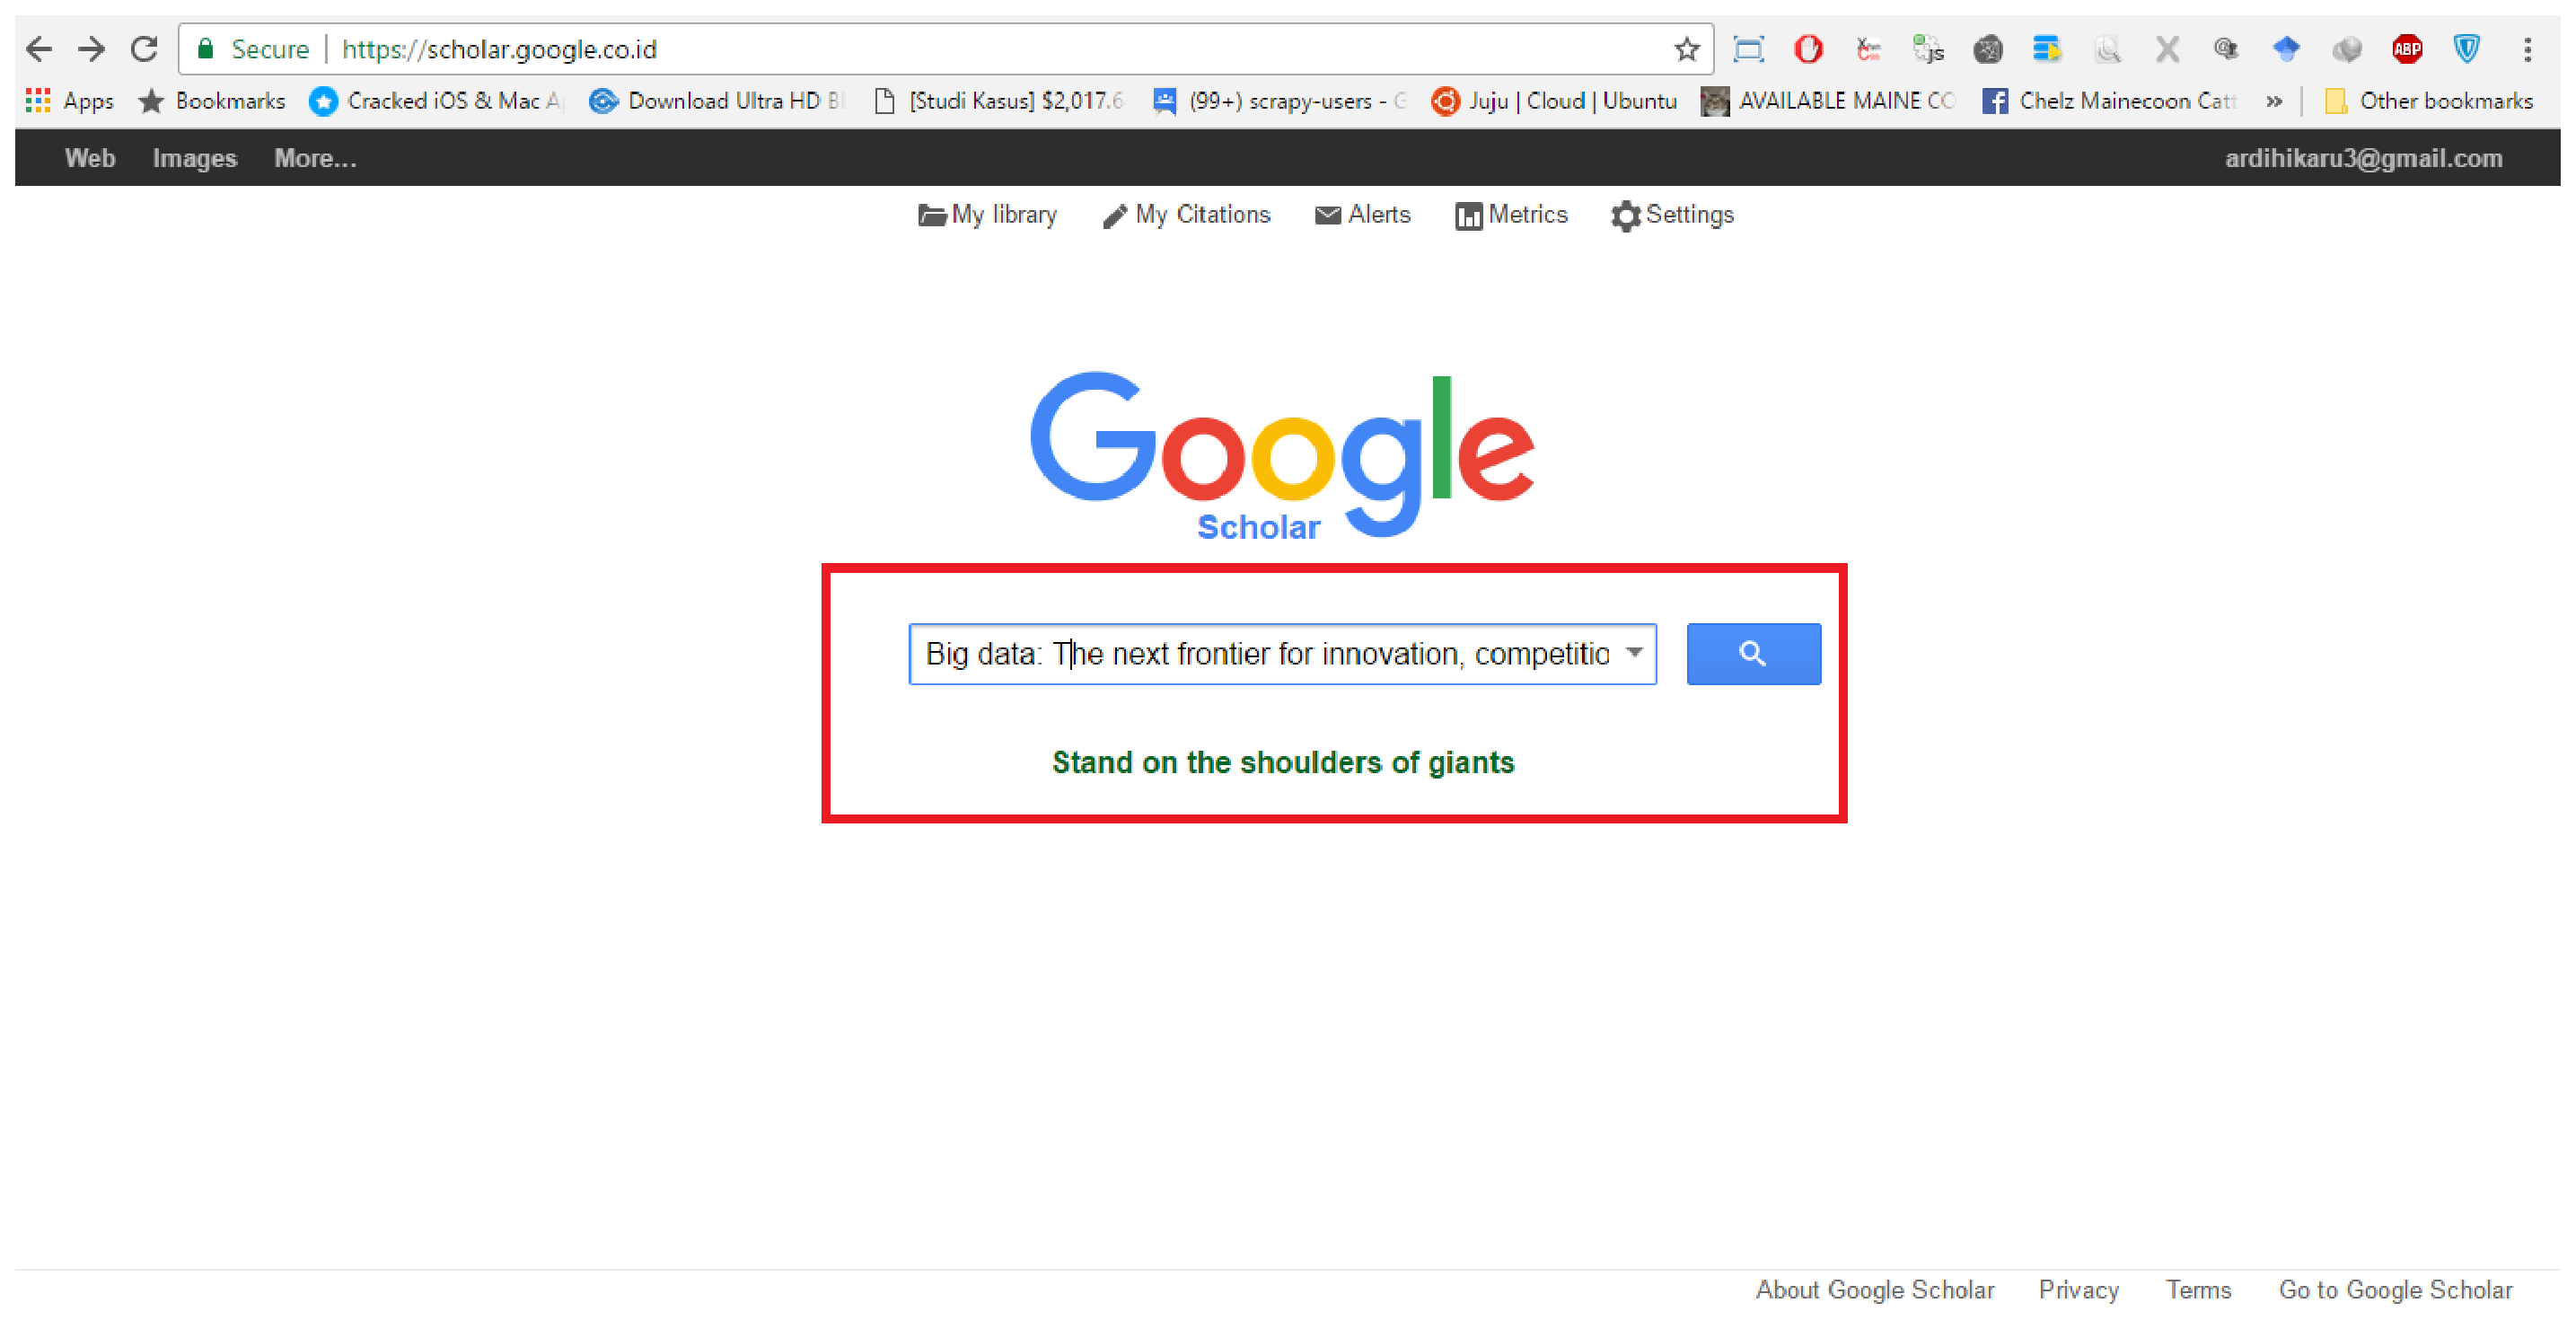
\includegraphics[width=120mm, height=120mm, keepaspectratio]{get_bib_script_part_1}
\caption{Buka Google Scholar}
\label{fig:fig3_1}
\end{figure}

\begin{figure}[H]
\centering
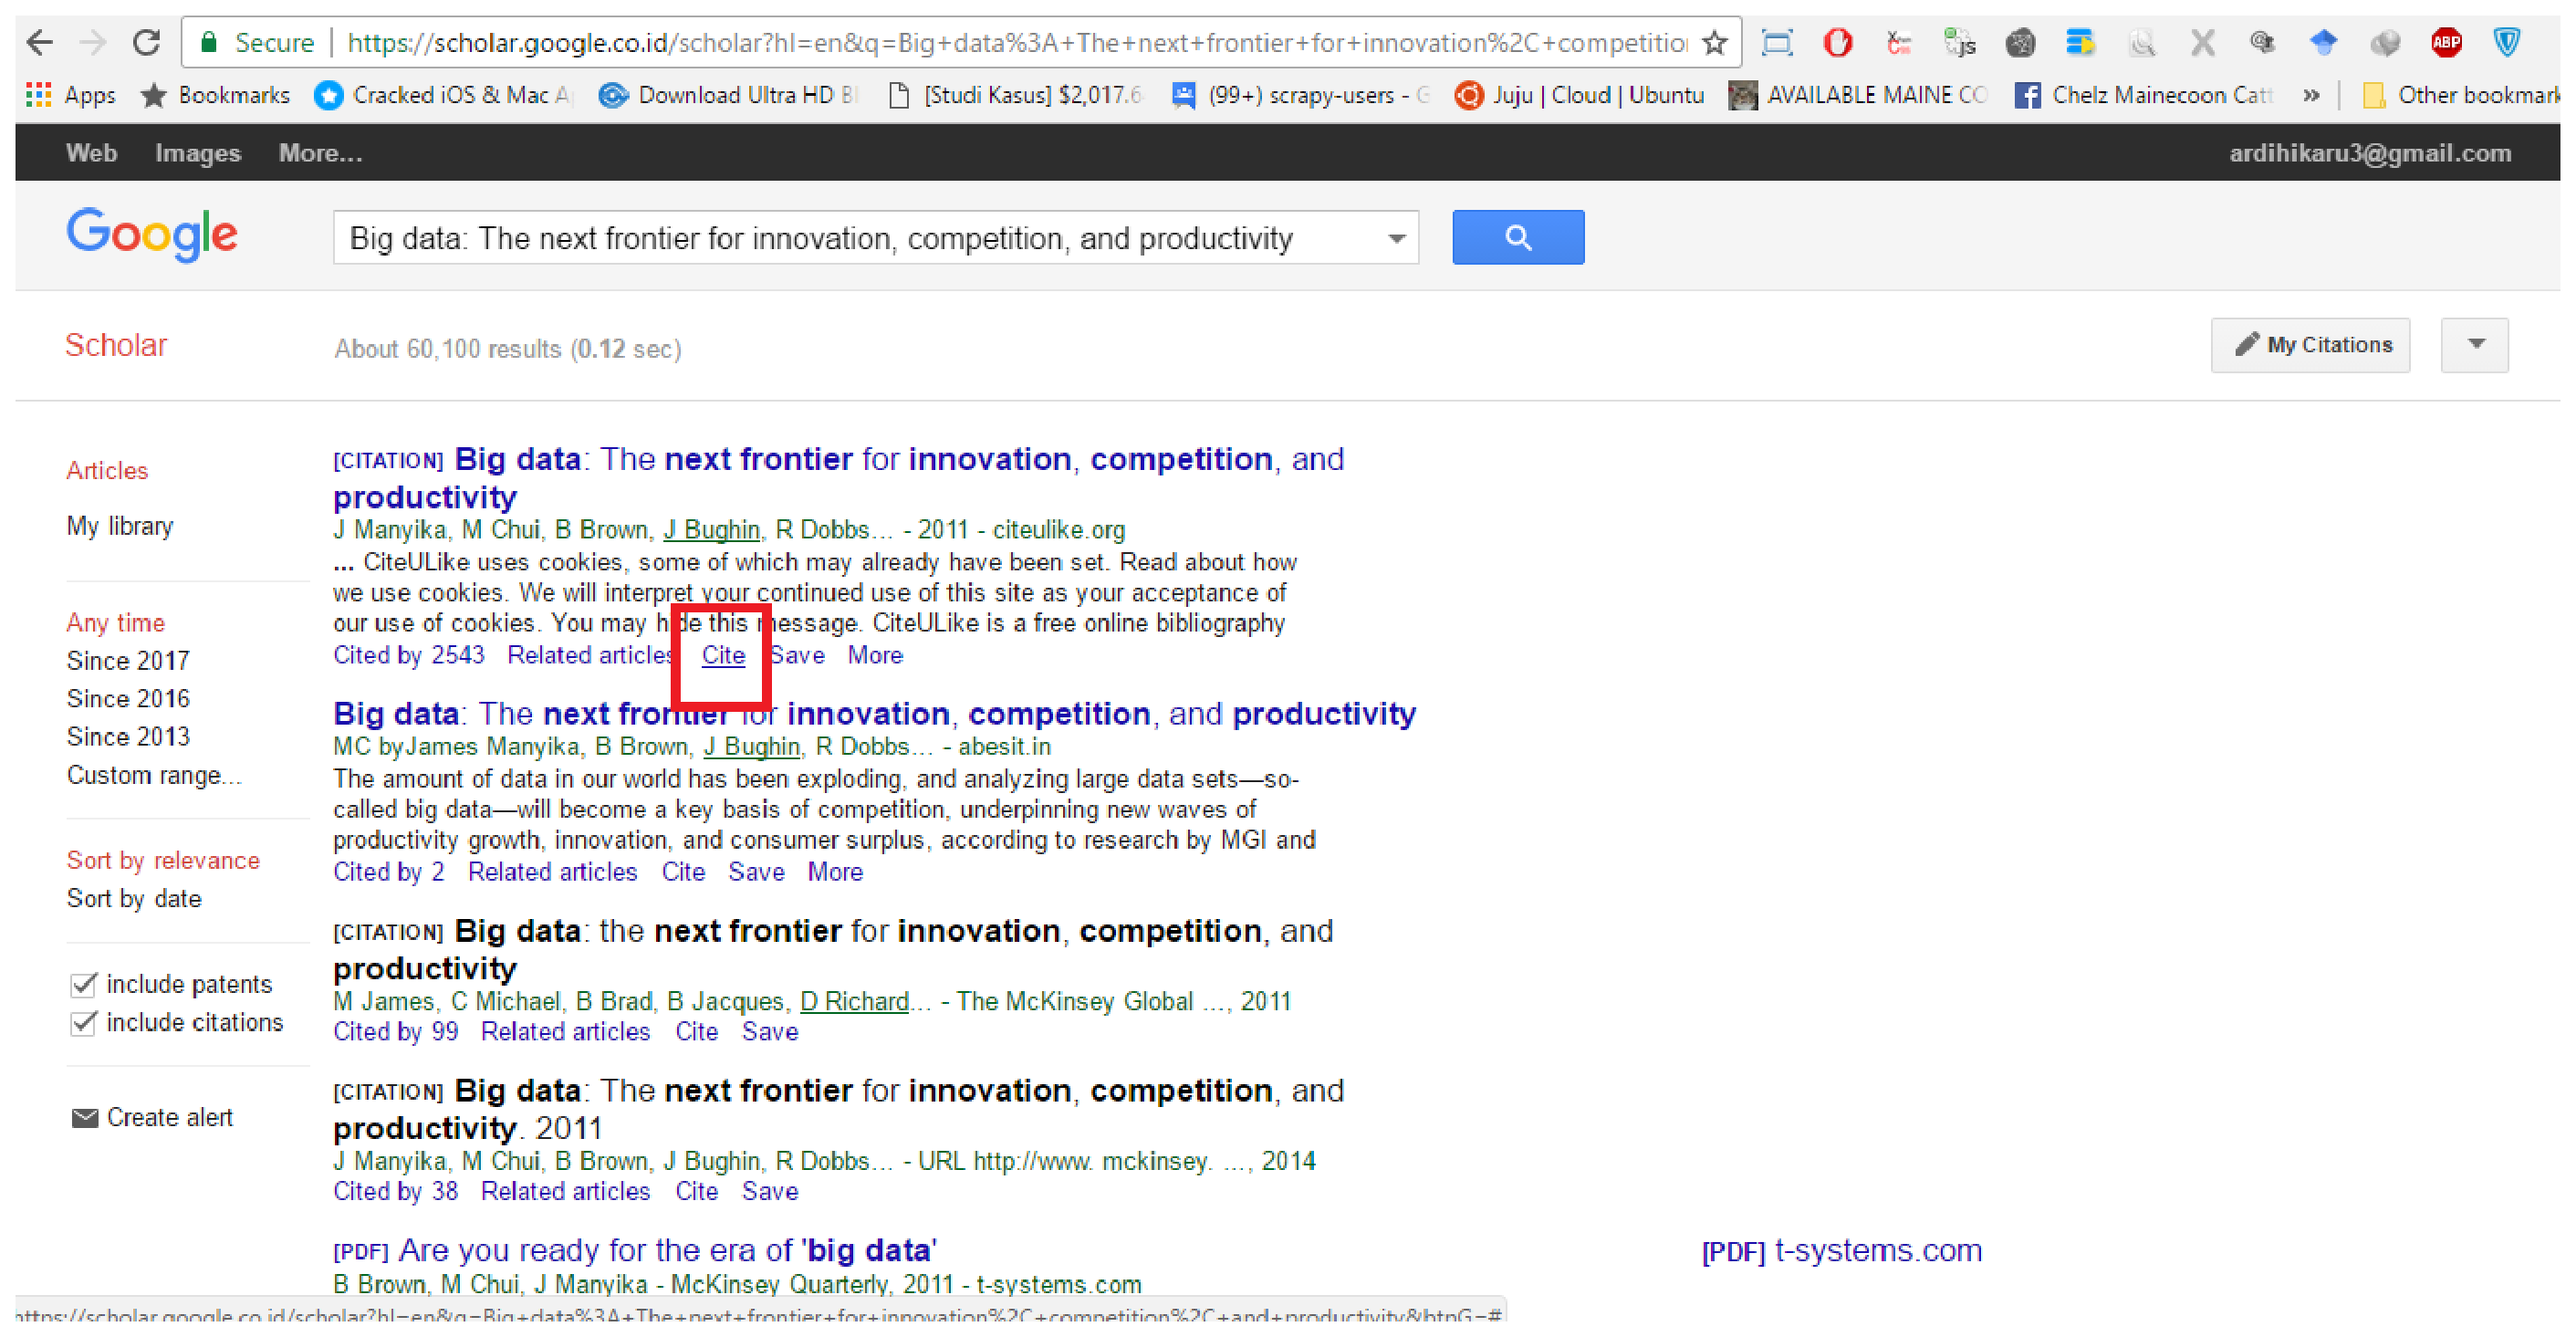
\includegraphics[width=120mm, height=120mm, keepaspectratio]{get_bib_script_part_2}
\caption{Click of the $Cite$ link.}
\label{fig:fig3_2}
\end{figure}

\begin{figure}[H]
\centering
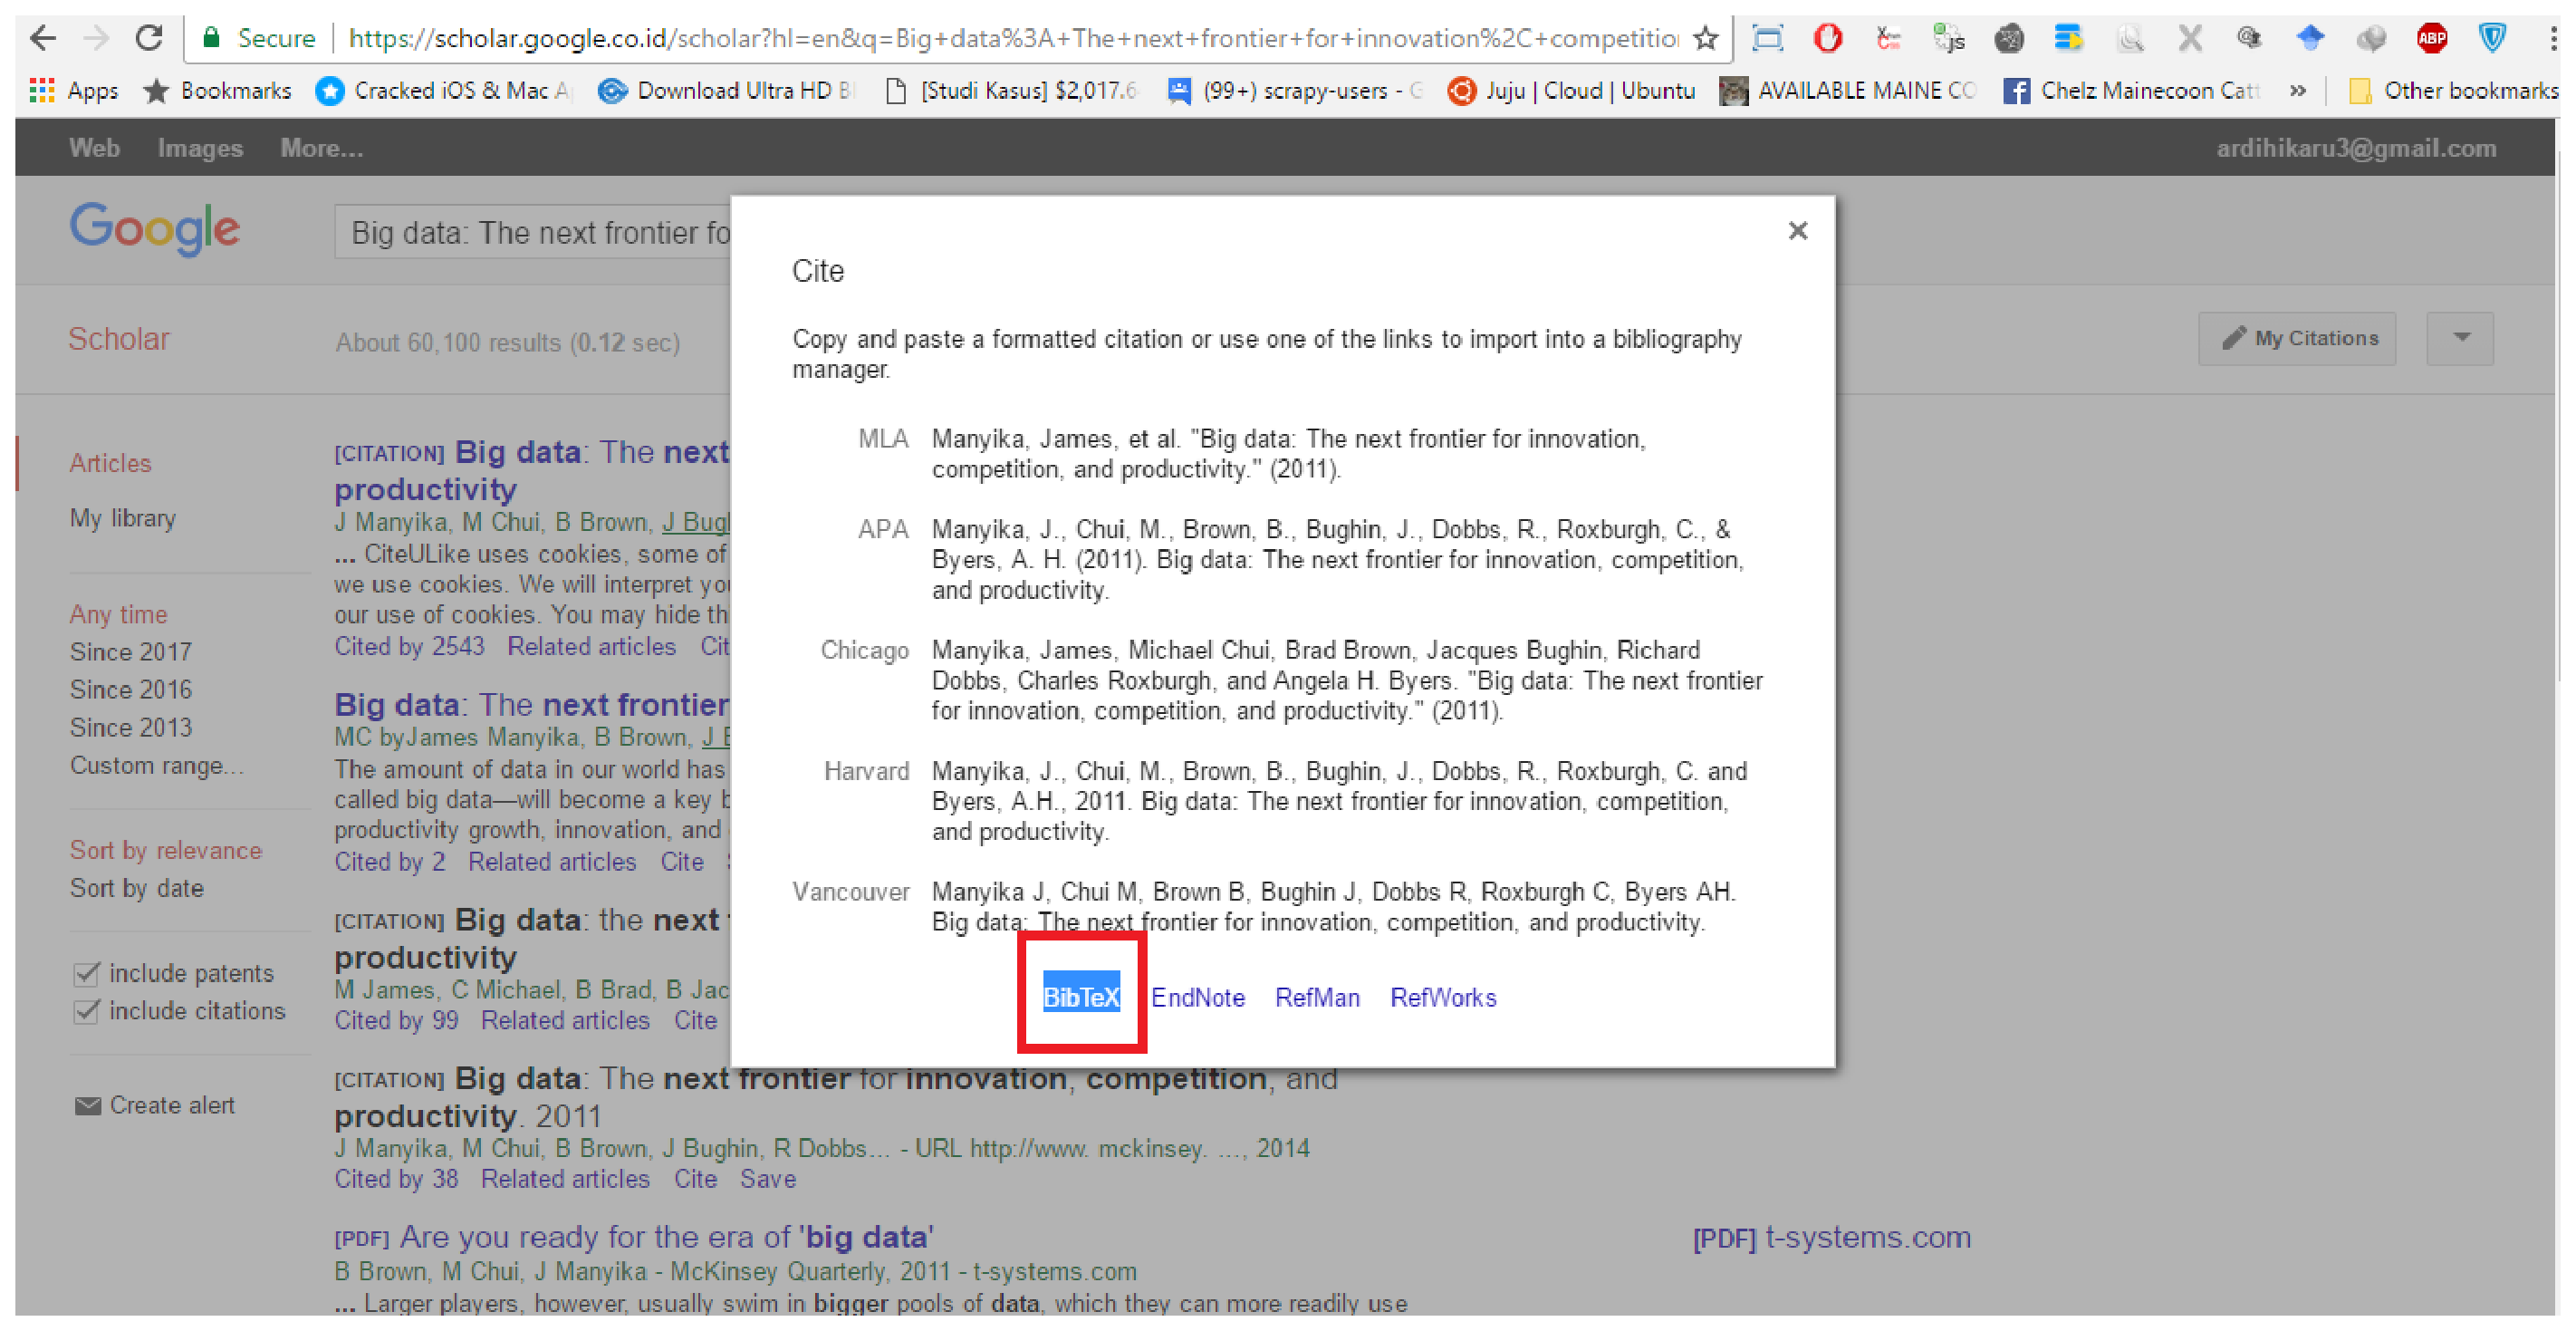
\includegraphics[width=120mm, height=120mm, keepaspectratio]{get_bib_script_part_3}
\caption{Click of the $BibTeX$ link.}
\label{fig:fig3_3}
\end{figure}

\begin{figure}[H]
\centering
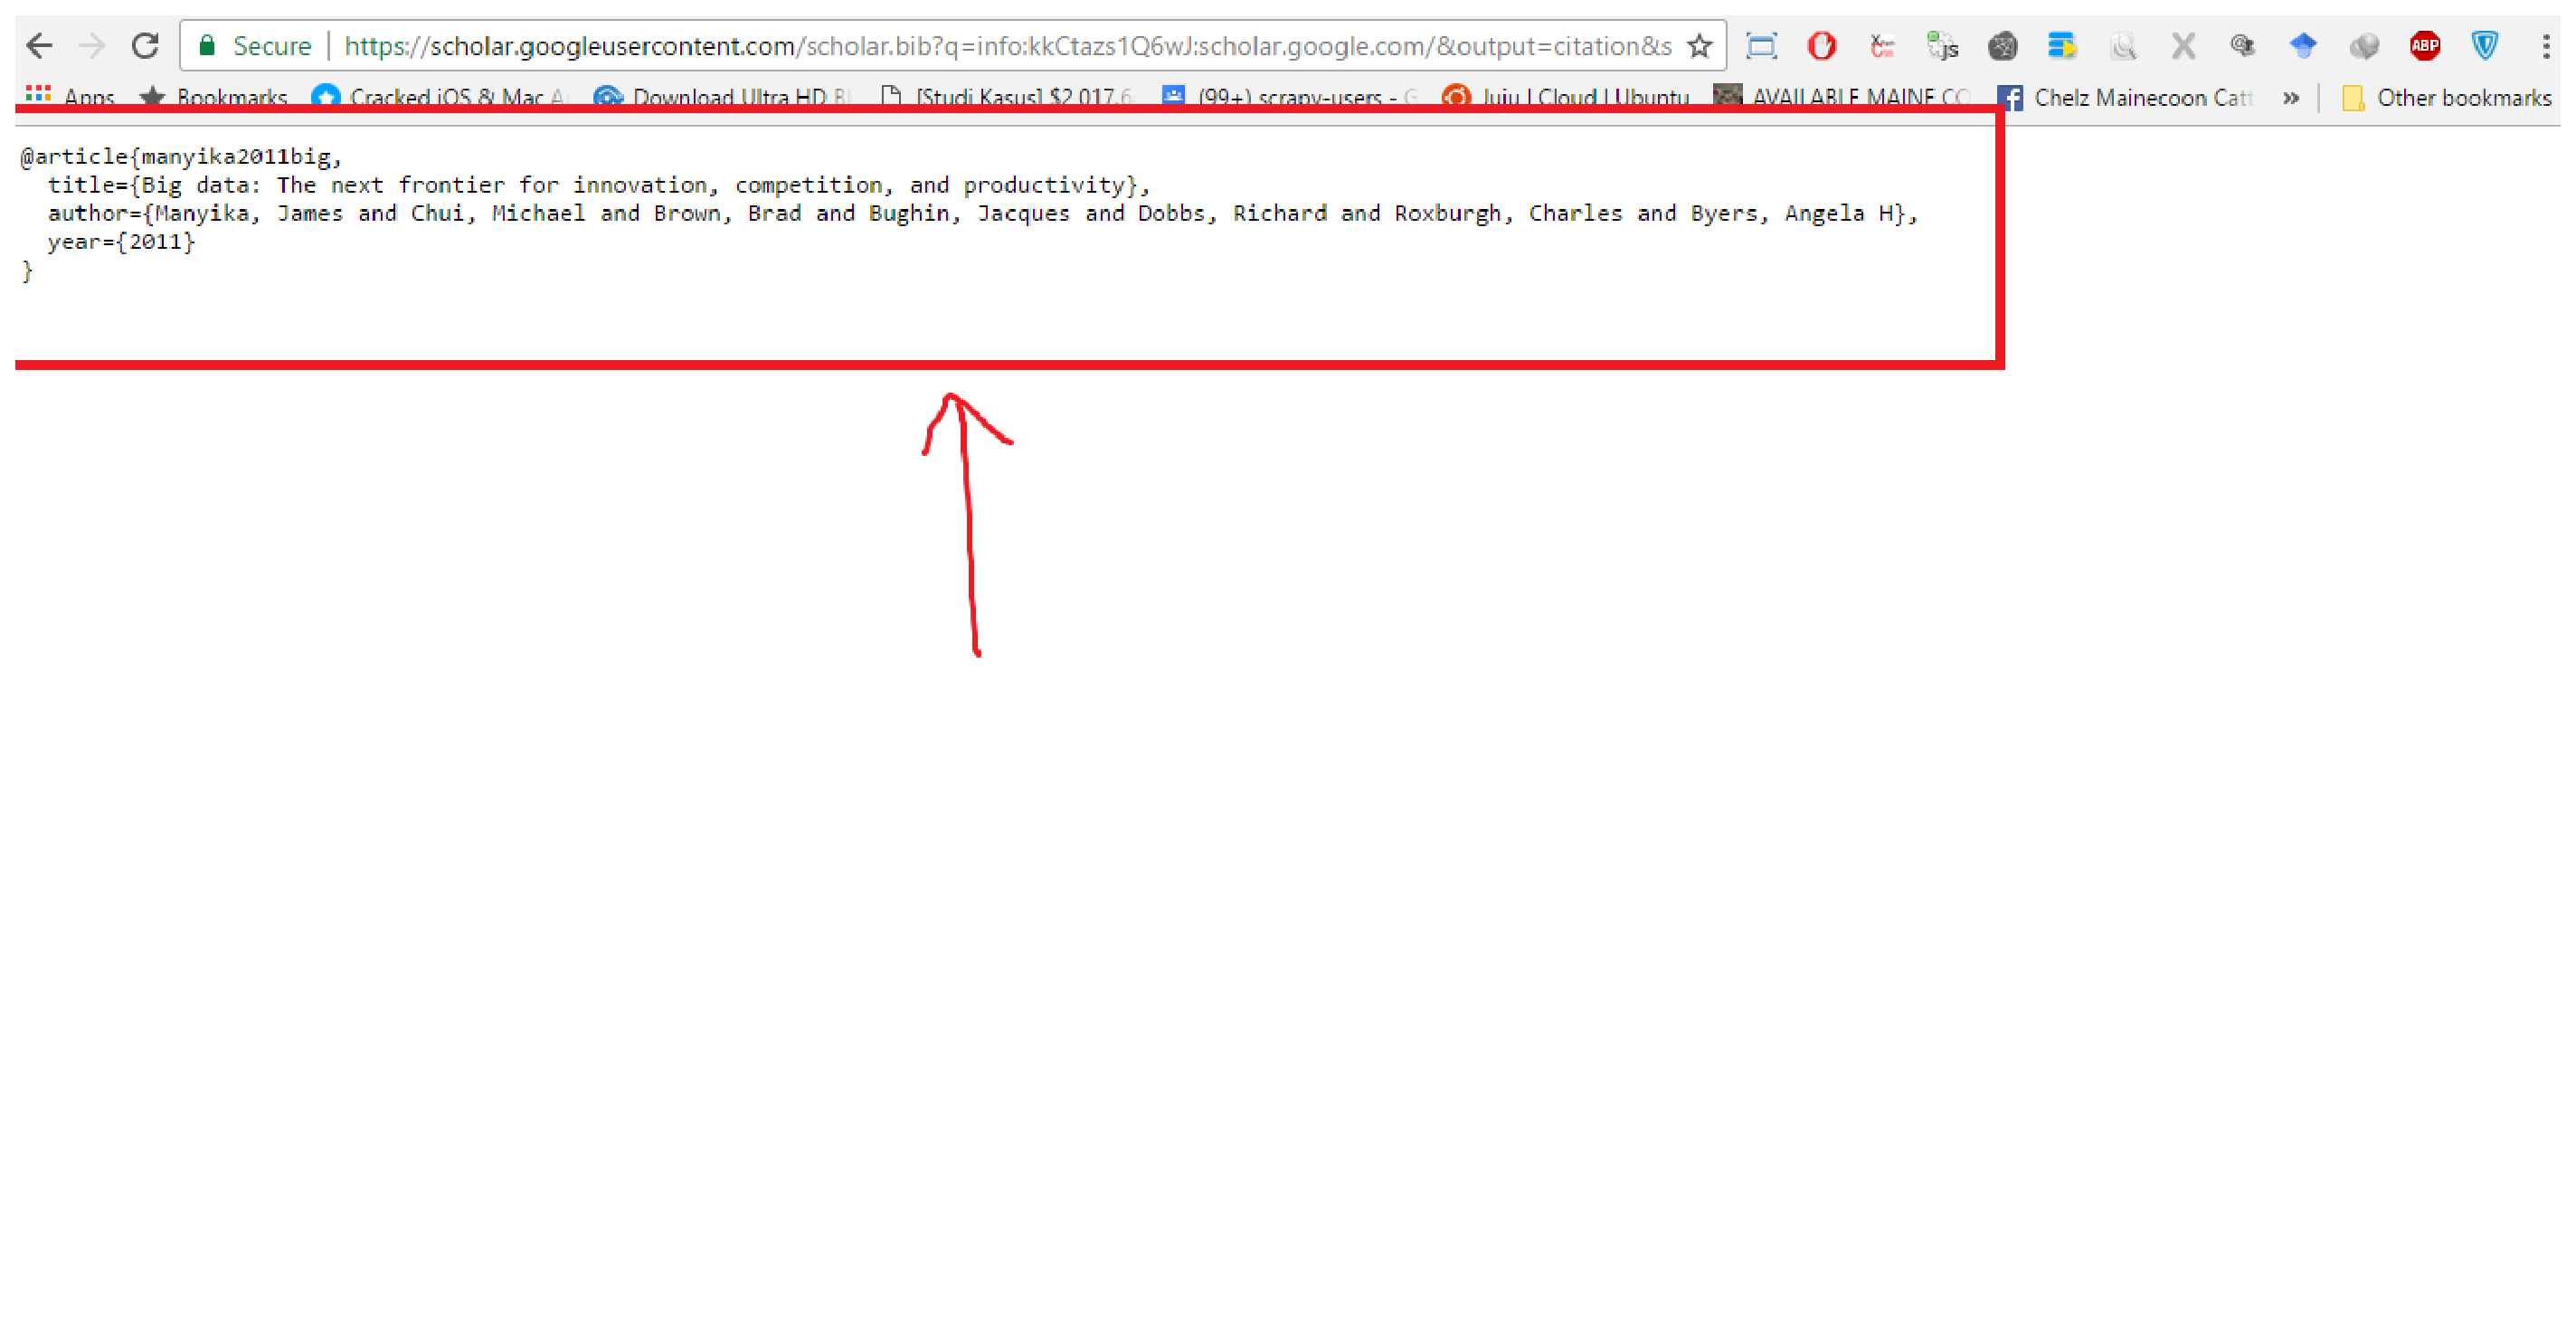
\includegraphics[width=120mm, height=120mm, keepaspectratio]{get_bib_script_part_4}
\caption{Copy the text}
\label{fig:fig3_4}
\end{figure}

For URL type references, you may check on one of my example of the $mybib.bib$ file. Once again, there are lots of alternative ways to write in LaTeX file. 